\documentclass[18pt,a4paper]{article}
\usepackage[letterpaper]{geometry}
\geometry{verbose,tmargin=2cm,bmargin=2cm,lmargin=2.50cm,rmargin=2.50cm}
%\usepackage[spanish]{babel}
\usepackage[utf8x]{inputenc}
%\usepackage[latin1]{inputenc}
\usepackage{amsmath,amsthm,amssymb,amsfonts,amstext}
\usepackage[pdftex]{graphicx}
\usepackage{caption}
\usepackage{subcaption}
\usepackage{framed}
\usepackage{wrapfig}
\DeclareGraphicsExtensions{.bmp,.png,.pdf,.jpg}
\setcounter{tocdepth}{3}
\usepackage{textcomp}
\usepackage{tikz}
\usepackage{circuitikz}
\usetikzlibrary{decorations.pathmorphing,patterns}
\usepackage{pgf}
\usepackage{multicol}
\usepackage{lipsum}
\usepackage{mathabx}
\usepackage{microtype}
\usepackage{vwcol}
\usepackage{pdflscape} % landscape specific pages
\usepackage{verbatim}
\usepackage{enumerate}
\usepackage{setspace}
\onehalfspacing
%\decimalcomma
%\deactivatequoting

%\renewcommand{\contentsname}{Contenido} % Renombrar a Español
%\renewcommand{\figurename}{Figura}
%\renewcommand{\tablename}{Tabla}
%\renewcommand{\refname}{Bibliografía}

\begin{document}

\begin{framed}
\begin{center}
%	\begin{multicols}{2}
%		\begin{minipage}{\textwidth}
%\begin{flushleft} 
{\bf \large {Stochastic optimization algorithms, 2016}}\\
		{\large\noindent\em\bf Report, Home Problems set2}\\
		Jose Esteban Pérez-Hidalgo, 880416T670

%\end{flushleft}
%\end{minipage}
	%	~
              %\includegraphics[width=0.2\textwidth]{/home/esteban/Dropbox/Public/image001.jpg}

  %      ~			
 %             %\includegraphics[width=0.2\textwidth]{/home/esteban/Dropbox/Public/image004.jpg}
		
%	\end{multicols}
\end{center}
\end{framed}

\section*{Problem 2.1 TSP}

\begin{enumerate}[a)]

	\item Here we are dealing with permutations of $N$ elements. So, the number of ways in which one can arrange $N$ (different) elements, say, the number of permutations, is the factorial of the number of elements, e.g: $N!$\\
	Now, in this particular case, we are looking for the number of {\it distinct paths}. Taking into account the paths one can form starting in different cities but running through the cities in the same order or the reverse order; for every distinct path ($d_p$) there are $2N$ ways to reorder the path keeping its path length.\\ Hence:
	$$d_p \times 2N = N!$$
	$$\Rightarrow d_p = \dfrac{N!}{2N} = \dfrac{(N - 1)!}{2}$$  
	
	\item As discussed during the lectures, the GA without modifications is not the best way to find the best solution for the TSP. In this case the algorithm was initialized with a population of $5000$ individuals.
	
	\item The ASO seems to be the proper way to attack the TSP. It takes many runs to find the best set of parameters to find the best solution. In this case the algorithm was initialized with a population of $50$ ants, $\alpha = 4$, $\beta = 3$ and $\rho = 0.5$. \\The parameters set was chosen based on the performance of the algorithm. A small number of ants was better than a large one, a medium value of $\rho$ worked well, and for $\alpha$ and $\beta$ it was noted that the algorithm reached a lower best path length faster with this values.\\
	Additional functions named: {\tt GetProbability.m}, {\tt GetNode.m} and {\tt EuclideanPathLength.m}; were used to solve this problem.
%\newpage
	
	\item The modifications made to the GA actually made the algorithm better at trying to find the best path, but the program gets stuck very early in the runs with a good but not optimal solution.\\
	Plots:
	
	\begin{figure}[h]
		\centering
		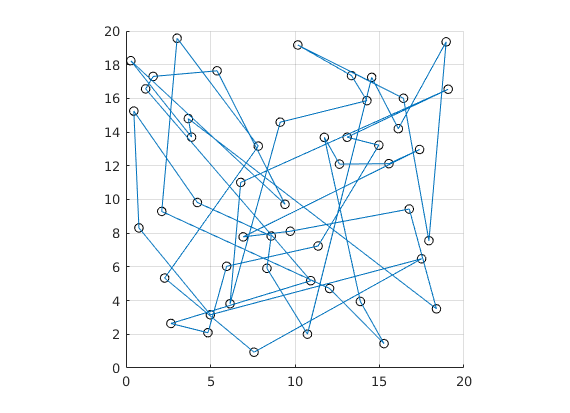
\includegraphics[width=0.4\textwidth]{GA21b351.png}
		\caption{\label{fig:1} Best path found using {\tt GA21b.m}. Path length = $351$ length units.}
	\end{figure}

\newpage

	\begin{figure}[h]
		\centering
		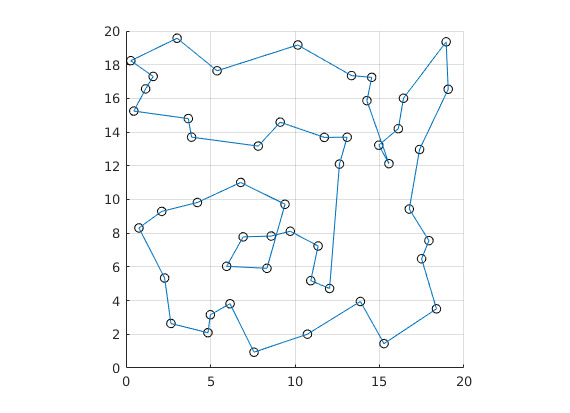
\includegraphics[width=0.6\textwidth]{PT128.png}
		\caption{\label{fig:2} Best path found using {\tt AntSystem.m}. Path length = $128$ length units.}
	\end{figure}

	\begin{figure}[h]
		\centering
		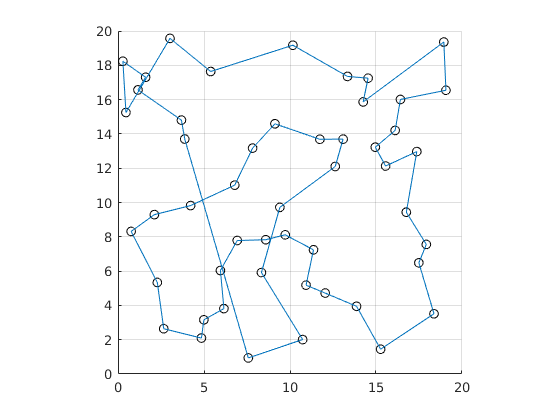
\includegraphics[width=0.6\textwidth]{21d13468.png}
		\caption{\label{fig:3} Best path found using {\tt GA21d.m}. Path length = $134$ length units.}
	\end{figure}
	
	The conclusion is that the ASO works better for this kind of problem, but it has to be noted that a lot of runs are needed to set the algorithm with the right choice of parameters.
	
\end{enumerate}

\newpage

\section*{Problem 2.2 PSO}
	\begin{enumerate}[a)]

		\item The algorithm handled this problem very well as the solution is reached very quickly (after 1000 generations). The minimum of the function is: 
		$$f(x^*,y^*) = 1$$
		Where:
		$$(x^*, y^*)^T = (\,5,4\,)^T.$$
				
		\item As in the previous case, the solution is reached very quickly (after 1000 generations). The minimum of the function is: 
		$$f^* = -737$$
		This global minimum is reached in two points:
		$${\mathbf x^*_a} = (\,0, 12, 23, 17, 6\,)^T.$$
		$${\mathbf x^*_b} = (\,0, 11, 22, 16, 6\,)^T.$$
		
	\end{enumerate}
	
	In both cases the PSO algorithm found the solution very quickly, proving the power of this method for this kind of problems
	
\end{document}
